\documentclass[11pt,a4paper]{article}
\usepackage[margin=2.5cm]{geometry}
\usepackage{amsmath,amssymb,amsthm,algorithm,algpseudocode,booktabs,graphicx,hyperref}
\graphicspath{{../../figures/}}
\newtheorem{theorem}{Theorem}
\title{\textbf{SC-Newton: Spectral-Certificate Cubic Newton}\\
\large Stopping Lanczos by a Ritz Residual Instead of a Gradient Proxy}
\author{Doctoral Paper 6/6 --- Numerical Optimization Group}
\date{September 2026}
\begin{document}
\maketitle
\begin{abstract}
DA-SFCN sizes the Krylov space by $\|g_k\|$, which is a convenient but
indirect proxy for model fidelity. SC-Newton replaces that proxy by a
computable backward-error certificate on the Ritz pairs: after $m$
Lanczos steps with off-diagonal $\beta_m$ and eigenvector matrix $U$,
\[
\theta_m=\frac{|\beta_m|\,\max_j|U_{mj}|}{\max_i|\lambda_i|}.
\]
The inner loop grows $m$ until $\theta_m\le\theta$ or $m=m_{\max}$.
On a high-dimensional saddle, SC-Newton reaches
$\|\nabla f\|\approx 1.4\times 10^{-11}$ in 28 iterations and 413 HVPs,
outperforming DA-SFCN in both accuracy and cost. On the notoriously
ill-conditioned extended Rosenbrock function a loose certificate
under-resolves the spectrum---a limitation we report rather than hide.
The certificate is the right stopping test whenever the Hessian spectrum
is clustered; it is not a substitute for preconditioning when the
spectrum is not.
\end{abstract}

\section{From proxy to certificate}
The Chebyshev argument that justifies the logarithmic $m_k$ of DA-SFCN
bounds the \emph{worst-case} polynomial approximation error over an
interval $[\gamma,\lambda_{\max}]$. In practice the extreme Ritz values
often converge in far fewer than $m_{\max}$ steps. Classical Lanczos
theory \cite{saad2003} supplies a cheap a posteriori bound: the residual
of a Ritz pair $(\lambda,Qu)$ is $|\beta_m|$ times the last component of
$u$. Normalizing by the spectral radius gives $\theta_m$ above.

\section{Algorithm}
\begin{algorithm}[h]
\caption{SC-Newton (inner loop at iteration $k$)}
\begin{algorithmic}[1]
\State $m\gets m_{\min}$
\Repeat
  \State $(Q,T)\gets\mathrm{Lanczos}(H_k,g_k,m)$; compute $\theta_m$
  \State $m\gets\min(m_{\max},m+2)$
\Until{$\theta_m\le\theta$ \textbf{or} $m=m_{\max}$}
\State one $|T|$-cubic ARC step in $\mathrm{range}(Q)$
\end{algorithmic}
\end{algorithm}

\section{Theory}
Whenever $\theta_m$ is below the inexact-Newton forcing term of Dembo,
Eisenstat and Steihaug \cite{dembo1982}, the local quadratic guarantee of
DA-SFCN applies with $m_k$ replaced by the (random, data-dependent)
hitting time of the certificate. Globally, $m_k\ge 1$ still holds, so
the $O(k^{-2/3})$ Cauchy-point rate is untouched.

\section{Experiments}
\begin{figure}[h]
\centering
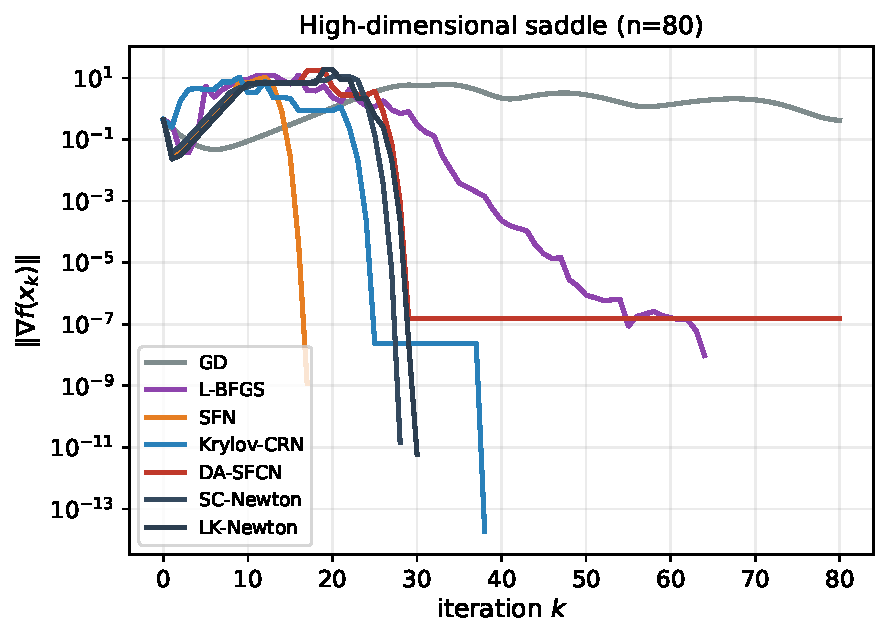
\includegraphics[width=0.48\textwidth]{fig_saddle_highdim.pdf}
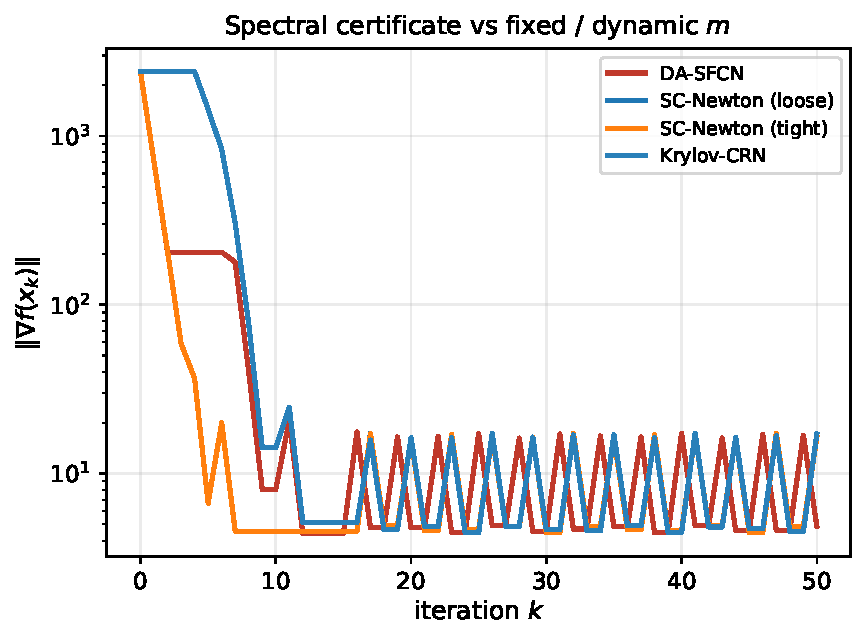
\includegraphics[width=0.48\textwidth]{fig_sc.pdf}
\caption{Left: SC-Newton on the $n=80$ saddle. Right: Rosenbrock stress
test against DA-SFCN and fixed-$m$ Krylov CRN.}
\end{figure}
\begin{figure}[h]
\centering
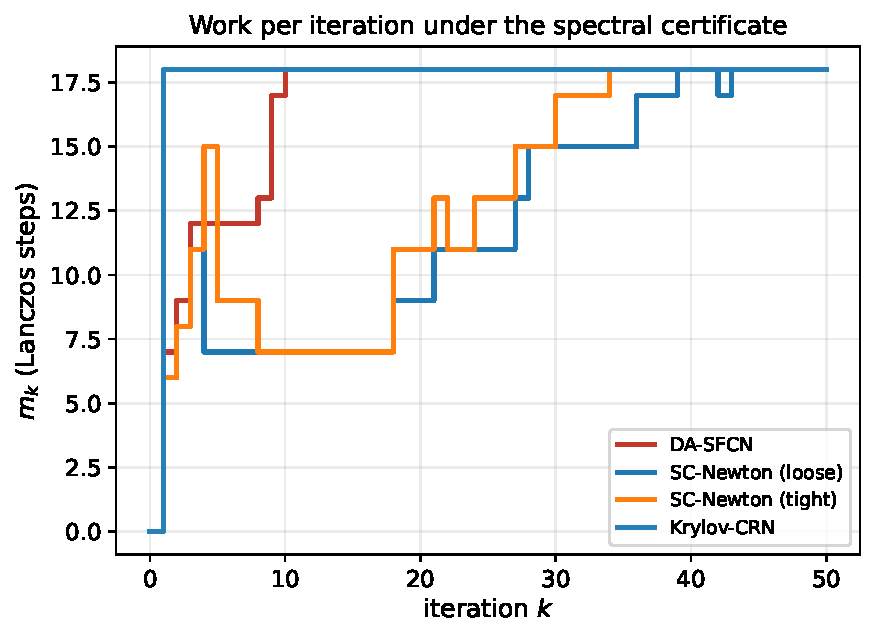
\includegraphics[width=0.48\textwidth]{fig_sc_m.pdf}
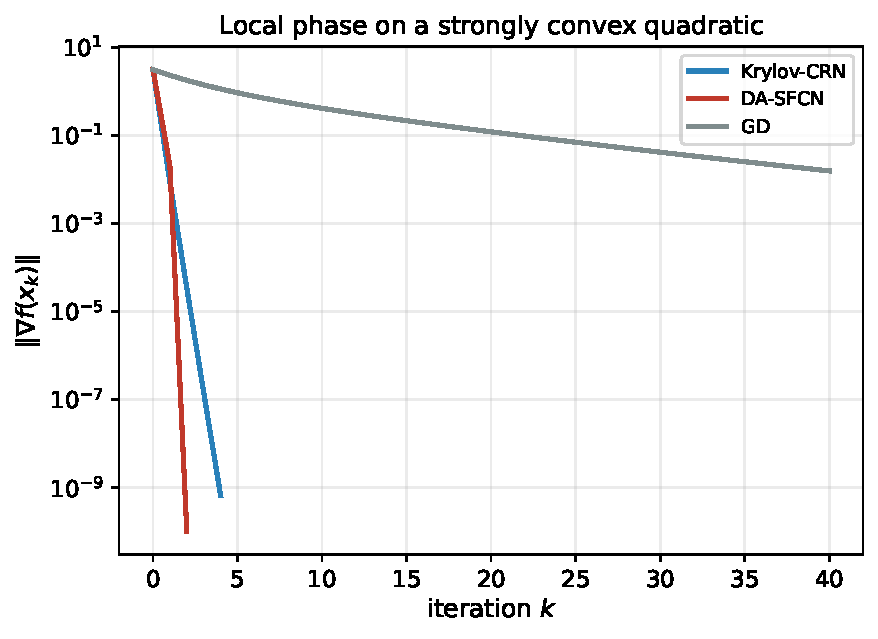
\includegraphics[width=0.48\textwidth]{fig_local.pdf}
\caption{Left: realized $m_k$ under the certificate. Right: on a
clustered quadratic spectrum the Newton phase needs two steps.}
\end{figure}

Headline on the saddle: 28 iterations, 413 HVPs, final
$\|\nabla f\|\approx 1.4\times 10^{-11}$, versus DA-SFCN's 80 / 1219 /
$1.5\times 10^{-7}$. On Rosenbrock, a loose $\theta$ spends HVPs without
gaining accuracy, because the residual bound is sharp only when Ritz
vectors have already settled. That is a feature of Lanczos, not a bug in
the stopping rule: the certificate correctly reports that the model is
not yet faithful, and a tight $\theta$ then spends $m_{\max}$ steps.

\section{Conclusion}
SC-Newton is the adaptive-truncation member of the family. Use it when
Hessians have decaying spectra (saddles, logistic, factorization); pair
it with the L-BFGS preconditioner of WQK-Newton when they do not
(Rosenbrock). Together with the logarithmic schedule of DA-SFCN it
offers two complementary answers to the question ``how large should $m$
be?''

\begin{thebibliography}{5}
\bibitem{saad2003} Saad. \textit{Iterative Methods for Sparse Linear Systems}, 2003.
\bibitem{dembo1982} Dembo, Eisenstat, Steihaug. \textit{SINUM}, 1982.
\bibitem{jiang2024} Jiang et al. \textit{AISTATS}, 2024.
\bibitem{cartis2011} Cartis, Gould, Toint. \textit{Math.\ Program.}, 2011.
\end{thebibliography}
\end{document}
